%!TEX encoding = UTF-8 Unicode
%!TEX root = ../compendium2.tex

\section{ScalaIDE och Eclipse}\label{appendix:ide:eclipse}

Eclipse%
\footnote{\href{https://en.wikipedia.org/wiki/Eclipse_(software)}{en.wikipedia.org/wiki/Eclipse\_(software)}}
är en professionell IDE som stödjer många olika programmeringsspråk. Eclipse är skriven i Java och bygger vidare på ett utvecklingsprojekt som initierades av IBM. Eclipse är ett fritt och öppet projekt som numera kontrolleras av en oberoende stiftelse.

Till Eclipse finns en insticksmodul \Eng{plug-in} som kallas ScalaIDE och erbjuder stöd för Scala med tillhörande standardbibliotek.

Eclipse är en omfattande och avancerad programmeringsmiljö med många funktioner och inställningar. Det finns även en omfattande uppsättning insticksmoduler och tilläggsprogram som underlättar utveckling av t.ex. webbprogram, databaser och mycket annat.

I detta avsnitt ges länkar till installation samt tips om hur du kommer igång med att använda Eclipse och ScalaIDE. Det går ganska snabbt att lära sig grunderna, men det kräven en viss ansträngning att lära sig de mer avancerade funktionerna. Det finns omfattande resurser på nätet som hjälper dig vidare.


\subsection{Installera ScalaIDE}\label{appendix:ide:eclipse:install}

Eclipse med ScalaIDE är förinstallerat på LTH:s datorer och startas med kommandot \texttt{scalaide} i ett terminalfönster.
För att installera ScalaIDE på din egen dator, följ nedan instruktioner:

\begin{enumerate}
\item Kontrollera enligt avsnitt \ref{appendix:compile:check-jdk} att du har \texttt{java} installerat och installera vid behov JDK enligt avsnitt \ref{appendix:compile:install-jdk}.

\item Installera senaste version av ScalaIDE (i skrivande stund v4.7.0 för Eclipse Oxygene och Scala 2.12.3) från denna sida:  \url{http://scala-ide.org/download/sdk.html} \\
Följ dessa steg:
\begin{enumerate}
\item Klicka på den variant som passar ditt operativsystem.
\item Filen som laddas ner heter något som liknar (beroende på OS): \\ till exempel  \emph{Windows 64-bit}
\\ Det kan ta ett tag att ladda ner filen som är på ca 280MB.

\item Dubbelklicka på filen för att packa upp den, vilket kan ta många minuter. Du får, när up	packningen är klar, ett bibliotek med namnet \code{eclipse} med en fungerande Eclipse-installation som du kan placera var du vill.
\end{enumerate}

\item Kör igång ScalaIDE första gången för att se så det fungerar genom att dubbelklicka på den exekverbara filen som ligger i underbiblioteket \texttt{eclipse}. I Windows heter den \texttt{eclipse.exe} medan den exekverbara filen i Linux heter \texttt{eclipse} utan filändelse.

% \item För Ubuntu Linux finns kompletterande installationsanvisningar här, som beskriver hur man kan skapa en ikon i app-menyn m.m.:
% \\ \url{http://askubuntu.com/questions/26632/how-to-install-eclipse}
% \\ Instruktionerna för Linux å länken ovan är nedan anpassade för version 4.6.1 av ScalaIDE som en serie kommandon att köra i terminalen. Adressen är hämtad från \url{http://scala-ide.org/download/sdk.html} genom att högerklicka på nedladdningsknappen och välja kopiering av adressen. Denna adress står efter \code{wget} nedan (anpassa adressen vid behov till nyare version om sådan kommit sedan detta skrevs). Klistra in ett kommando i taget och kontrollera att det inte blir några fellmeddelande. Nedladdningen med \texttt{wget} kan ta ett tag.
% \begin{verbatim}
% $ cd ~/Downloads
% $ wget http://downloads.typesafe.com/scalaide-pack/\
% 4.6.1-vfinal-neon-212-20170609/scala-SDK-4.6.1-vfinal-\
% 2.12-linux.gtk.x86_64.tar.gz
% $ tar -zxvf scala-SDK-4.6.1-vfinal-2.12-linux.gtk.x86_64.tar.gz
% $ sudo mv ~/Downloads/eclipse /opt/scalaide46  # ändra 46 vid behov
% $ cat > ~/Desktop/scalaide.desktop <<EOF
% [Desktop Entry]
% Name=ScalaIDE
% Type=Application
% Exec=env UBUNTU_MENUPROXY=0 scalaide
% Terminal=false
% Icon=scalaide
% Comment=Integrated Development Environment
% NoDisplay=false
% Categories=Development;IDE;
% Name[en]=ScalaIDE
% EOF
% $ chmod +x ~/Desktop/scalaide.desktop
% $ sudo ln -s /opt/scalaide46/eclipse /usr/local/bin/scalaide
% $ sudo desktop-file-install ~/Desktop/scalaide.desktop
% $ sudo cp /opt/scalaide46/icon.xpm /usr/share/pixmaps/scalaide.xpm
% \end{verbatim}
\end{enumerate}


\subsection{Använda ScalaIDE och Eclipse}\label{appendix:ide:eclipse:use}

Ett grundläggande koncept i Eclipse är \textbf{workspace}. Ett workspace utgör ett arbetsområde kopplat till en katalog i ditt filsystem där du kan arbeta med ett eller flera \textbf{projekt}. Ett projekt innehåller i sin tur dina källkodsfiler och klassfiler etc. i en specifik katalogstruktur som Eclipse skapar när du editerar, kompilerar och kör dina projekt.

\subsubsection{Starta och välja workspace}\label{subsubsection:start:eclipse}

När du startar Eclipse måste du välja vilket workspace du vill använda innan du kommer vidare. När du kör igång Eclipse första gången, klicka OK enligt det förslag som ges. Du kan senare växla workspace genom menyn \MenuArrow{File}\Menu{Switch Workspace}. Om katalogen du anger inte redan finns, kommer den att skapas och initieras med de filer Eclipse behöver.

% I figur \ref{fig:appendix:eclipse:welcome} visas välkomstfliken i Eclipse med sina länkar till funktionsöversikt och olika handledningar. Stäng välkomstfliken genom att klicka på flikens kryss eller på ikonen \textit{Workbench}. Då kommer du vidare till den normala arbetsytan i Eclipse. Du kan få tillbaka välkomstfliken igen via menyn \MenuArrow{Help}\Menu{Welcome}.
%
% \begin{figure}[H]
% \centering
% 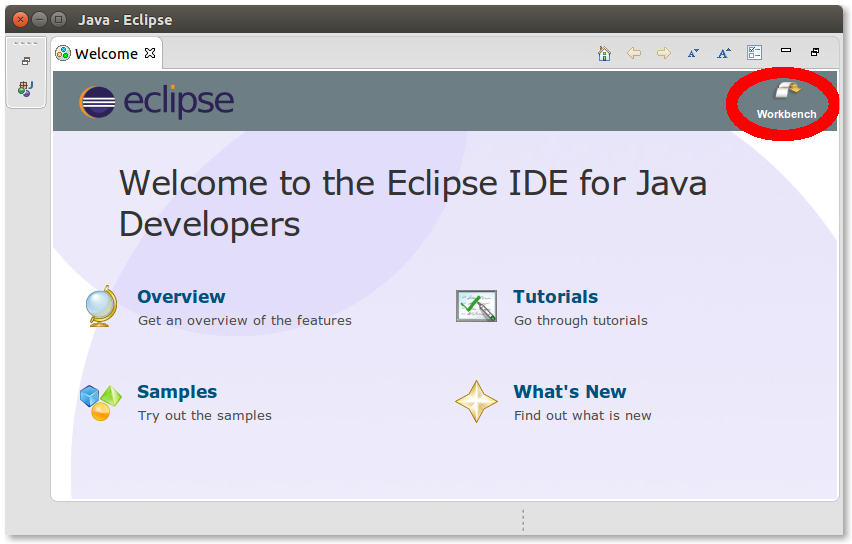
\includegraphics[width=1.0\textwidth]{../img/eclipse/eclipse-welcome.png}
% \caption{Välkomstfliken för Eclipse, som nås via menyn \MenuArrow{Help}\Menu{Welcome}. Gå vidare genom att klicka på \textit{Workbench}.}
% \label{fig:appendix:eclipse:welcome}
% \end{figure}

\subsubsection{Välja perspektiv och visa olika vyer}

Eclipse-fönstret kan innehålla många underfönster i olika flikar, så kallade \textbf{views} eller vyer, som kan arrangeras på olika vis efter hur du vill ha dem. Vilka vyer som syns och hur de placeras beror på vilket s.k. \textbf{perspective} som är aktivt.  Figur \ref{fig:appendix:eclipse:open-perspective} visar arbetsytan med olika vyer i Scala-perspektivet.

Stäng vyn \textit{Outline} om du vill ha mer plats till de övriga vyerna för paketnavigering, editering och utdata. Du kan öppna stängda vyer igen genom menyn \MenuArrow{Window}\Menu{Show View}.
Du kan även återställa perspektivet om din vy blivit konstig med \MenuArrow{Window}\MenuArrow{Perspective}\MenuArrow{Reset Perspective...}

Om du vill anpassa arbetsytan för Java kan du byta perspektiv med klick på 
\includegraphics[scale=0.75]{../img/eclipse/eclipse-perspective-button.png} eller genom menyn \MenuArrow{Window}\MenuArrow{Perspective}\MenuArrow{Open Perspective}\MenuArrow{Other...}\Menu{Java}.

\begin{figure}
\centering
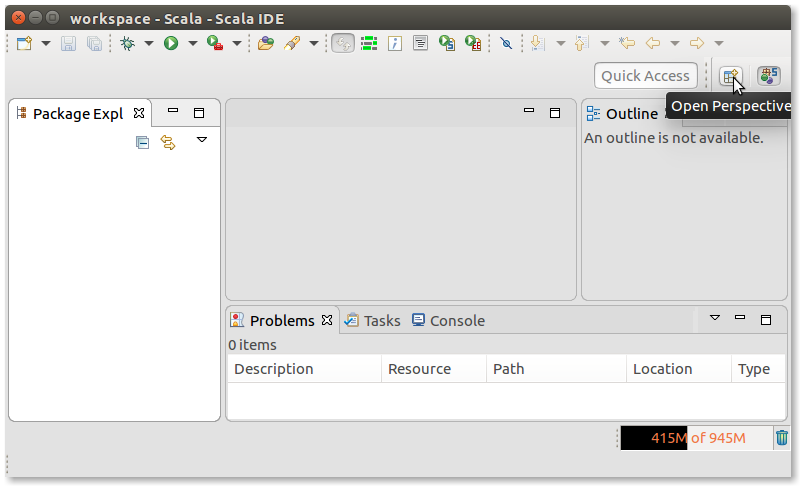
\includegraphics[width=1.0\textwidth]{../img/eclipse/eclipse-scala-perspective.png}
\caption{Arbetsytan i Eclipse. Du kan växla mellan Scala-perspektivet och andra perspektiv, t.ex. Debug-perspektivet eller Java-perspektivet genom att klicka på knappen \Menu{Open Perspective}.}
\label{fig:appendix:eclipse:open-perspective}
\end{figure}

\subsubsection{Hello World}\label{subsubsection:eclipse:hello-world}

Efter att du öppnat ScalaIDE i ett tomt workspace med Scala-perspektivet enligt föregående avsnitt, kan du skapa ditt första projekt med ett \textit{''Hello World''}-program enligt stegen nedan.

\begin{enumerate}
\item Högerklicka i \Menu{Package Explorer} och välj \MenuArrow{New}\Menu{Scala Project}, varefter en dialogruta visas.

\item Fyll i namnet \texttt{hello} i fältet \Menu{Project Name} och klicka \Button{Finish}. Vänta tills skapandet av projektet är klart enligt notifieringar i fönstrets nederkant.

\item Högerklicka igen i \Menu{Package Explorer} och välj \MenuArrow{New}\Menu{Scala Object}, varefter en ny dialogruta visas.

\item Fyll i namnet \texttt{hi} i fältet \Menu{Name} och klicka \Button{Finish}.

\item Du får nu i editorvyn ett kodskelett med \code{object hi}.

\item Börja skriv \code{main} som visas i figur \ref{fig:appendix:eclipse:complete-main} och tryck Ctrl+Mellanslag för att aktivera kodkomplettering \Eng{code completion}. Då får du upp en lista med många alternativ. Välj alternativet \texttt{main - main} varefter ett kodskelett med en main-metod klistras in automatiskt i din kod.

\begin{figure}
\centering
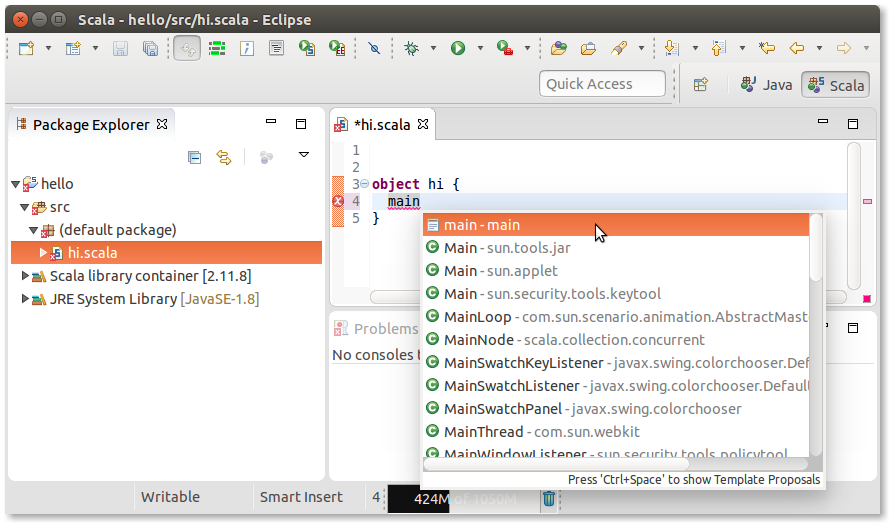
\includegraphics[width=1.0\textwidth]{../img/eclipse/eclipse-complete-main.png}
\caption{Aktivera kodkomplettering med Ctrl+Mellanslag efter ordet \code{main}.}
\label{fig:appendix:eclipse:complete-main}
\end{figure}

\item Fyll i lämplig utskriftstext i ett \code{println}-anrop så att din \code{main}-metod blir så som visas i editorfliken i figur \ref{fig:appendix:eclipse:hello-world}.

\begin{figure}[H]
\centering
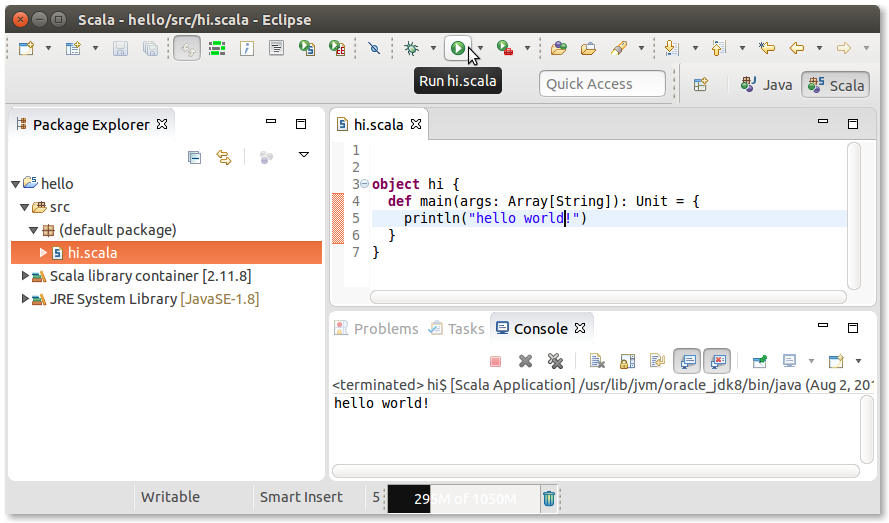
\includegraphics[width=1.0\textwidth]{../img/eclipse/eclipse-hello-world.png}
\caption{Skriv klart \code{main}-metoden och kör ditt program med play-knappen.}
\label{fig:appendix:eclipse:hello-world}
\end{figure}

\item Kör ditt program genom att klicka på den lilla ner-pilen som finns \emph{bredvid} den gröna play-knappen, som muspekaren i figur \ref{fig:appendix:eclipse:hello-world} pekar på. Då vecklas en meny ut där du kan välja \MenuArrow{Run As...}\Menu{Scala Application}. Eller så kan du höger-klicka på filen \texttt{hi.scala} och välja \MenuArrow{Run As...}\Menu{Scala Application}. Detta behöver du bara göra första gången och då skapas en s.k. \textit{Run Configuration}. Du kan sedan trycka Ctrl+F11 för att köra igång din app enligt senaste \textit{Run Configuration} eller klicka på den gröna play-knappen.

\item Du kan öppna din \textit{Run Configuration} genom menyn  \MenuArrow{Run}\Menu{Run Configurations...} och där ställa in många saker, bland annat vilka argument som ska ges till \code{main}-metoden under fliken \textit{Arguments} i textrutan \textit{Program Arguments}.

\end{enumerate}



\subsection{Anpassa ScalaIDE och Eclipse}\label{subsection:appendix:ide:eclipse:tweaks}

\newcommand\EclipsePrefs{\MenuArrow{Window}\MenuArrow{Preferences}}
\newcommand\EclipsePrefsGeneral{\EclipsePrefs\MenuArrow{General}}


%Förutom maxminneshöjningen i filen \texttt{eclipse.ini}, som finns i installationskatalogen för Eclipse, till minst \texttt{-Xmx1G}
Det kan vara bra att göra några ytterligare anpassningar av Eclipse och ScalaIDE enligt nedan. Du hittar inställningarna i menyn \EclipsePrefs ... uppe till höger i Eclipse-fönstret.

\begin{enumerate}
% \item \EclipsePrefsGeneral
% \\ Markera \FramedCheckmark{Show Heap Status} så får du se minnesanvändningen i en liten ruta i nederdelen av fönstret, vilket hjälper dig att upptäcka om minnesbegränsningen i filen \texttt{eclipse.ini} är en flaskhals vid stora projekt och många öppna fönster. Klicka sedan \Button{Apply} längst ner.

% \item \label{item:scala-perspective} \EclipsePrefsGeneral\MenuArrow{Editors}\MenuArrow{Perspectives}
% \\ Markera \textit{Scala} i listan med perspektiv och klicka på knappen
%  \\ \Button{Make default} till höger och sedan på knappen \Button{Apply} längst ner.

\item \EclipsePrefsGeneral\MenuArrow{Editors}\MenuArrow{TextEditors}
\\ Markera \FramedCheckmark{Insert spaces for tabs} så att du slipper specialtecken som kan tolkas olika av olika editorer. Klicka sedan \Button{Apply} längst ner.

\item \EclipsePrefsGeneral\MenuArrow{Editors}\MenuArrow{TextEditors}
\\ \MenuArrow{Spelling} Avmarkera \FramedUnchecked{Enable spell checking} för att slippa att svenska namn och svenska kommentarer markeras som felstavade. Om du senare jobbar med ett projekt helt på engelska, kan du med fördel markera denna kryssruta igen. Klicka sedan \Button{Apply} längst ner.

\item \EclipsePrefsGeneral\MenuArrow{Editors}\MenuArrow{Webbrowser}
\\ Markera \FramedCheckmark{Use external web browser} för att köra din vanliga webbläsare när du klickar på länkar. Klicka sedan \Button{Apply} längst ner.

\item  \EclipsePrefs\MenuArrow{Scala}\MenuArrow{Compiler}
\\ I fliken \textbf{Standard} markera dessa kryssrutor för att få extra varningar: \\
\begin{tabular}{l @{}l @{}l}
\textit{deprecation} & \FramedCheckmark{} & varnar vid användning av föråldrad kod som snart utgår \\
\textit{feature}     & \FramedCheckmark{} & påminner om import vid användning av avancerad kod  \\
\textit{unchecked}   & \FramedCheckmark{} & ger tips vid speciella problem med generiska typer \\
\end{tabular}\\
och klicka sedan på knappen \Button{Apply} längst ner.

\item \EclipsePrefs\MenuArrow{Java}\MenuArrow{Compiler}\MenuArrow{Errors/Warnings}
\\ Veckla ut listan \textbf{Potential programming problems} och sätt \textbf{Resource leak} till alternativet \textbf{Ignore}, så slipper du varningar vid användning \jcode{Scanner} i Java. Klicka sedan \Button{Apply} längst ner.

\end{enumerate}

\noindent Ovan anpassningar är rekommenderade men inte nödvändiga och du kan gärna välja att göra andra anpassningar som passar just dig. Skriv då gärna ner vilken inställning du ändrat, så att du hittar tillbaka om du ångrar dig.

%Du hittar tips om fler inställningar för att anpassa ScalaIDE här: \\
%\url{http://scala-ide.org/docs/current-user-doc/advancedsetup}






\subsubsection{Ladda ner kursens workspace och importera i Eclipse}\label{subsubsection:download--import-workspace}

Det finns en zip-fil med ett workspace med projekt för flera av kursens laborationer som du kan ladda ner och importera i Eclipse. Följ stegen nedan.

\begin{enumerate}
\item Ladda ner kursens workspace här: \url{http://cs.lth.se/pgk/ws}

\item Packa upp filen på lämpligt ställe, t.ex. i katalogen \texttt{eclipse/pgk/workspace/}

\item Starta Eclipse med ScalaIDE-plugin (se startinstruktioner på sidan \pageref{subsubsection:start:eclipse}).

\item Växla workspace till biblioteket du nyss packade upp, ungefär som i figur \ref{fig:eclipse:ide:open} och klicka \Button{OK}.

\begin{figure}[H]
\centering
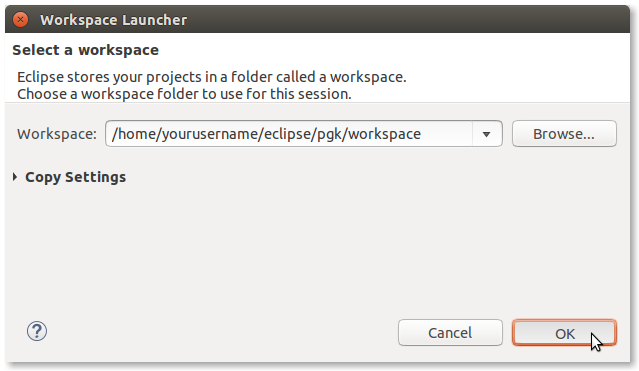
\includegraphics[width=0.8\textwidth]{../img/eclipse/eclipse-select-workspace.png}
\caption {Öppna kursens workspace genom att bläddra till biblioteket där du packade upp filen som du laddat ned från: \url{http://cs.lth.se/pgk/ws} \\Om du redan har ett annat workspace öppet, man du växla workspace med menyn \MenuArrow{File}\MenuArrow{Switch Workspace}\Menu{Other...}}
\label{fig:eclipse:ide:open}
\end{figure}

\item
%Stäng välkomstfliken för att komma vidare till workbench (se figur \ref{fig:appendix:eclipse:welcome} på sidan \pageref{fig:appendix:eclipse:welcome}).
Det ska nu se ut ungefär som i figur~\ref{fig:appendix:eclipse:open-perspective} på sidan \pageref{fig:appendix:eclipse:open-perspective}. Det syns ännu inget i \textit{Package Explorer} då vi ännu inte importerat något projekt.

\item Innan du går vidare, säkerställ att du har Scala-perspektivet aktiverat. Du kan växla till Scala-perspektivet genom att trycka på 
\includegraphics[scale=0.75]{../img/eclipse/eclipse-perspective-button.png} eller genom menyn \MenuArrow{Window}\MenuArrow{Perspective}\MenuArrow{Open Perspective}\MenuArrow{Other...}\Menu{Scala}.
%Du kan anpassa inställningarna så att Scala blir \textit{default perspective}, se steg \ref{item:scala-perspective} i avsnitt \ref{subsection:appendix:ide:eclipse:tweaks} på sidan \pageref{subsection:appendix:ide:eclipse:tweaks}.


\item Högerklicka i \textit{Package Explorer} och välj \Menu{Import...}, se Fig.~\ref{fig:eclipse:import}, eller välj menyn \MenuArrow{File}\Menu{Import...}.

\begin{figure}[h]
\centering
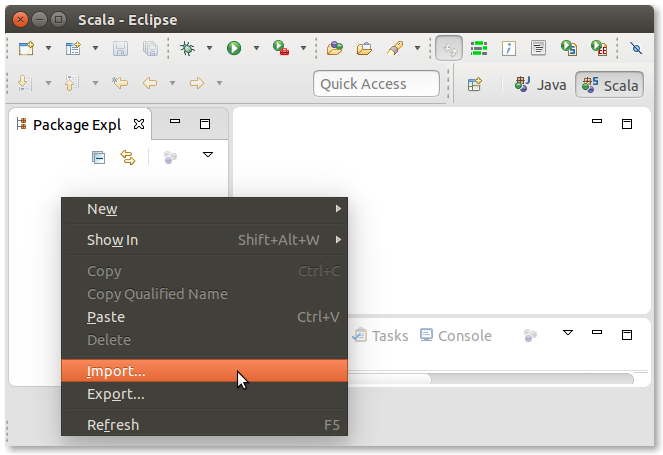
\includegraphics[width=0.9\textwidth]{../img/eclipse/eclipse-import.png}
\caption {Välj \Menu{Import}-menyn för att importera existerande projekt.}
\label{fig:eclipse:import}
\end{figure}

\item Nu öppnas \Menu{Import}-dialogen som visas i figur \ref{fig:eclipse:import-existing}. Öppna mappen \Menu{General}, markera \textbf{Existing Projects into Workspace} och klicka \Button{Next}.



\begin{figure}[h]
\centering
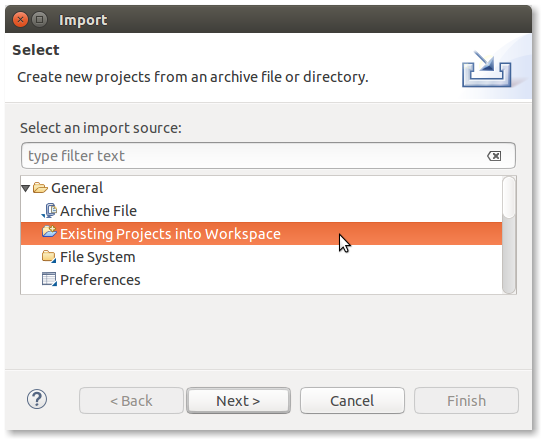
\includegraphics[width=0.6\textwidth]{../img/eclipse/eclipse-import-existing.png}
\caption {Välj att importera existerande projekt under \Menu{General}.}
\label{fig:eclipse:import-existing}
\end{figure}


\begin{figure}[h]
\centering
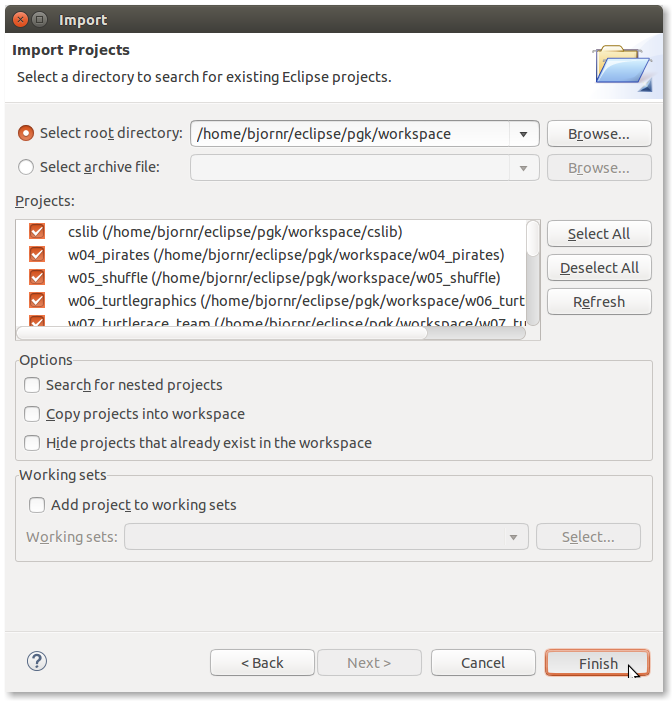
\includegraphics[width=0.85\textwidth]{../img/eclipse/eclipse-import-projects.png}
\caption {Välj \FramedCheckmark{Select Root Directory} (anpassa sökvägen till katalogen där lagt den uppackade katalogen med kursens workspace) och klicka \Button{Browse} och därefter \Button{Ok}. Då kommer biblioteken upp i listan som bilden ovan visar. Alla bibliotek ska vara förvalda. Avsluta med att klicka \Button{Finish}}
\label{fig:eclipse:import-projects}
\end{figure}

\item Nu kommer ytterligare ett dialogfönster som visas i figure \ref{fig:eclipse:import-projects}. Följ instruktionerna i bildtexten.

% \item Följ ''Hello World''-instruktionerna på sidan \pageref{subsubsection:eclipse:hello-world} och skapa programmet som visas i figure \ref{fig:eclipse:pirates-hi}, genom att veckla ut projektet \textbf{w04\_pirates}, markera och högerklicka på paketet \textbf{priates}, och välja \MenuArrow{New}\Menu{Scala Object}.

\item Efter att du klickat \Button{Finish} sätter ScalaIDE igång att bygga workspace i bakgrunden. Detta kan ta ett tag. Du kan följa bygget nere till höger i fönstret:
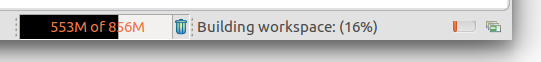
\includegraphics[width=0.75\textwidth]{../img/eclipse/scalaide-import-progress.png}

\item När bygget är klart kan du köra huvudprogrammet i laboration \texttt{w08\_life} genom att högerklicka på filen \texttt{src/main/scala/life/Main.scala} och välja \MenuArrow{Run As}\Menu{Scala Application}.

%\item Om du får problem, fråga någon som känner till Eclipse om hjälp. Det finns även mycket hjälp på nätet, se till exempel: \\ \href{http://stackoverflow.com/questions/8522149/eclipse-not-recognizing-scala-code}{stackoverflow.com/questions/8522149/eclipse-not-recognizing-scala-code}

% \begin{figure}[H]
% \centering
% 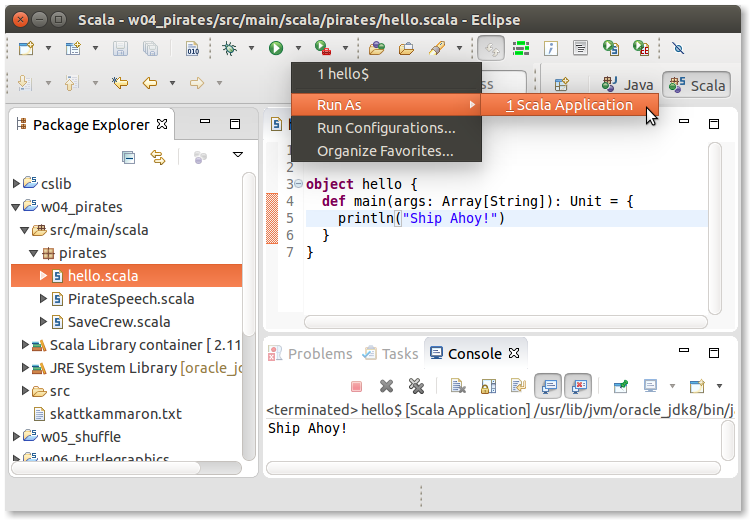
\includegraphics[width=1.0\textwidth]{../img/eclipse/eclipse-pirates-hello.png}
% \caption {Skapa ett \MenuArrow{New}\Menu{Scala Object} med kod enligt bilden.}
% \label{fig:eclipse:pirates-hi}
% \end{figure}


\end{enumerate}

%
% \subsection{Använda debuggern i ScalaIDE/Eclipse}
%
% !!! Läs först appendix \ref{appendix:debug}
%
% \subsubsection{Sätta brytpunkter i Eclipse}\TODO
% \subsubsection{Stegad exekvering i Eclipse}\TODO
% \subsubsection{Inspektera variabler i Eclipse}\TODO
